% Options for packages loaded elsewhere
\PassOptionsToPackage{unicode}{hyperref}
\PassOptionsToPackage{hyphens}{url}
\PassOptionsToPackage{dvipsnames,svgnames,x11names}{xcolor}
%
\documentclass[
  letterpaper,
  DIV=11,
  numbers=noendperiod]{scrartcl}

\usepackage{amsmath,amssymb}
\usepackage{iftex}
\ifPDFTeX
  \usepackage[T1]{fontenc}
  \usepackage[utf8]{inputenc}
  \usepackage{textcomp} % provide euro and other symbols
\else % if luatex or xetex
  \usepackage{unicode-math}
  \defaultfontfeatures{Scale=MatchLowercase}
  \defaultfontfeatures[\rmfamily]{Ligatures=TeX,Scale=1}
\fi
\usepackage{lmodern}
\ifPDFTeX\else  
    % xetex/luatex font selection
\fi
% Use upquote if available, for straight quotes in verbatim environments
\IfFileExists{upquote.sty}{\usepackage{upquote}}{}
\IfFileExists{microtype.sty}{% use microtype if available
  \usepackage[]{microtype}
  \UseMicrotypeSet[protrusion]{basicmath} % disable protrusion for tt fonts
}{}
\makeatletter
\@ifundefined{KOMAClassName}{% if non-KOMA class
  \IfFileExists{parskip.sty}{%
    \usepackage{parskip}
  }{% else
    \setlength{\parindent}{0pt}
    \setlength{\parskip}{6pt plus 2pt minus 1pt}}
}{% if KOMA class
  \KOMAoptions{parskip=half}}
\makeatother
\usepackage{xcolor}
\setlength{\emergencystretch}{3em} % prevent overfull lines
\setcounter{secnumdepth}{-\maxdimen} % remove section numbering
% Make \paragraph and \subparagraph free-standing
\ifx\paragraph\undefined\else
  \let\oldparagraph\paragraph
  \renewcommand{\paragraph}[1]{\oldparagraph{#1}\mbox{}}
\fi
\ifx\subparagraph\undefined\else
  \let\oldsubparagraph\subparagraph
  \renewcommand{\subparagraph}[1]{\oldsubparagraph{#1}\mbox{}}
\fi


\providecommand{\tightlist}{%
  \setlength{\itemsep}{0pt}\setlength{\parskip}{0pt}}\usepackage{longtable,booktabs,array}
\usepackage{calc} % for calculating minipage widths
% Correct order of tables after \paragraph or \subparagraph
\usepackage{etoolbox}
\makeatletter
\patchcmd\longtable{\par}{\if@noskipsec\mbox{}\fi\par}{}{}
\makeatother
% Allow footnotes in longtable head/foot
\IfFileExists{footnotehyper.sty}{\usepackage{footnotehyper}}{\usepackage{footnote}}
\makesavenoteenv{longtable}
\usepackage{graphicx}
\makeatletter
\def\maxwidth{\ifdim\Gin@nat@width>\linewidth\linewidth\else\Gin@nat@width\fi}
\def\maxheight{\ifdim\Gin@nat@height>\textheight\textheight\else\Gin@nat@height\fi}
\makeatother
% Scale images if necessary, so that they will not overflow the page
% margins by default, and it is still possible to overwrite the defaults
% using explicit options in \includegraphics[width, height, ...]{}
\setkeys{Gin}{width=\maxwidth,height=\maxheight,keepaspectratio}
% Set default figure placement to htbp
\makeatletter
\def\fps@figure{htbp}
\makeatother

\KOMAoption{captions}{tablesignature}
\makeatletter
\makeatother
\makeatletter
\makeatother
\makeatletter
\@ifpackageloaded{caption}{}{\usepackage{caption}}
\AtBeginDocument{%
\ifdefined\contentsname
  \renewcommand*\contentsname{Table des matières}
\else
  \newcommand\contentsname{Table des matières}
\fi
\ifdefined\listfigurename
  \renewcommand*\listfigurename{Liste des Figures}
\else
  \newcommand\listfigurename{Liste des Figures}
\fi
\ifdefined\listtablename
  \renewcommand*\listtablename{Liste des Tables}
\else
  \newcommand\listtablename{Liste des Tables}
\fi
\ifdefined\figurename
  \renewcommand*\figurename{Figure}
\else
  \newcommand\figurename{Figure}
\fi
\ifdefined\tablename
  \renewcommand*\tablename{Tableau}
\else
  \newcommand\tablename{Tableau}
\fi
}
\@ifpackageloaded{float}{}{\usepackage{float}}
\floatstyle{ruled}
\@ifundefined{c@chapter}{\newfloat{codelisting}{h}{lop}}{\newfloat{codelisting}{h}{lop}[chapter]}
\floatname{codelisting}{Listing}
\newcommand*\listoflistings{\listof{codelisting}{Liste des Listings}}
\makeatother
\makeatletter
\@ifpackageloaded{caption}{}{\usepackage{caption}}
\@ifpackageloaded{subcaption}{}{\usepackage{subcaption}}
\makeatother
\makeatletter
\@ifpackageloaded{tcolorbox}{}{\usepackage[skins,breakable]{tcolorbox}}
\makeatother
\makeatletter
\@ifundefined{shadecolor}{\definecolor{shadecolor}{rgb}{.97, .97, .97}}
\makeatother
\makeatletter
\makeatother
\makeatletter
\makeatother
\makeatletter
\@ifpackageloaded{fontawesome5}{}{\usepackage{fontawesome5}}
\makeatother
\ifLuaTeX
\usepackage[bidi=basic]{babel}
\else
\usepackage[bidi=default]{babel}
\fi
\babelprovide[main,import]{french}
% get rid of language-specific shorthands (see #6817):
\let\LanguageShortHands\languageshorthands
\def\languageshorthands#1{}
\ifLuaTeX
  \usepackage{selnolig}  % disable illegal ligatures
\fi
\IfFileExists{bookmark.sty}{\usepackage{bookmark}}{\usepackage{hyperref}}
\IfFileExists{xurl.sty}{\usepackage{xurl}}{} % add URL line breaks if available
\urlstyle{same} % disable monospaced font for URLs
\hypersetup{
  pdftitle={Exercices sur les graphes},
  pdflang={fr},
  colorlinks=true,
  linkcolor={blue},
  filecolor={Maroon},
  citecolor={Blue},
  urlcolor={Blue},
  pdfcreator={LaTeX via pandoc}}

\title{Exercices sur les graphes}
\usepackage{etoolbox}
\makeatletter
\providecommand{\subtitle}[1]{% add subtitle to \maketitle
  \apptocmd{\@title}{\par {\large #1 \par}}{}{}
}
\makeatother
\subtitle{S4 - Arbres et graphes}
\author{}
\date{}

\begin{document}
\maketitle
\ifdefined\Shaded\renewenvironment{Shaded}{\begin{tcolorbox}[boxrule=0pt, frame hidden, breakable, borderline west={3pt}{0pt}{shadecolor}, sharp corners, interior hidden, enhanced]}{\end{tcolorbox}}\fi

\emph{Les exercices précédés du symbole \faIcon{desktop} sont à faire
sur machine, en sauvegardant le fichier si nécessaire.}

\emph{Les exercices précédés du symbole \faIcon{pencil-alt} doivent être
résolus par écrit.}

\hypertarget{fa-solid-pencil-alt-exercice-1}{%
\subsection{\texorpdfstring{\faIcon{pencil-alt} Exercice
1}{ Exercice 1}}\label{fa-solid-pencil-alt-exercice-1}}

On dit qu'un graphe est \textbf{simple} s'il n'y a pas de boucle ni de
double arête. Un graphe simple est dit \textbf{complet} s'il est non
orienté et que chaque paire de sommets est reliée par une arête.

Dessiner un graphe complet d'ordre 3, puis un graphe complet d'ordre 4.

\hypertarget{fa-solid-pencil-alt-exercice-2}{%
\subsection{\texorpdfstring{\faIcon{pencil-alt} Exercice
2}{ Exercice 2}}\label{fa-solid-pencil-alt-exercice-2}}

\textbf{Graphe d'un réseau électrique}

Un de vos amis travaille pour un distributeur d'électricité.

Il doit proposer à son supérieur une représentation du réseau reliant
différentes villes. Comme il n'y arrive pas trop, il voudrait que vous
la lui fassiez.

Pour simplifier le problème, il a déjà renommé les villes en A, B, C, D,
E et F. De plus, il vous donne les informations suivantes :

\begin{itemize}
\tightlist
\item
  la ville B est reliée par un réseau électrique aux villes A, C et D,
\item
  la ville A est reliée par un réseau électrique aux villes B, E et F,
\item
  la ville C est reliée par un réseau électrique aux villes B, D, E et
  F,
\item
  la ville D est reliée par un réseau électrique aux villes B, C et F,
\item
  la ville E est reliée par un réseau électrique aux villes A, C et F,
\item
  la ville F est relié par un réseau électrique aux villes A, C, D et E.
\end{itemize}

Proposer un graphe qui modélise la situation.

Ce graphe est-il complet ? Pourquoi ?

Donner sa matrice d'adjacence.

\hypertarget{fa-solid-pencil-alt-exercice-3}{%
\subsection{\texorpdfstring{\faIcon{pencil-alt} Exercice
3}{ Exercice 3}}\label{fa-solid-pencil-alt-exercice-3}}

Voici un ensemble de relations :

\begin{itemize}
\tightlist
\item
  A est ami avec tout le monde sauf G,
\item
  B est ami avec A, D et H,
\item
  C est ami avec A, F, G et H,
\item
  D est ami avec A, B et H,
\item
  E est ami avec A et H,
\item
  F est ami avec A et C,
\item
  G est ami avec C et H,
\item
  H est ami avec A, B, C, D, E et G.
\end{itemize}

\begin{enumerate}
\def\labelenumi{\arabic{enumi}.}
\tightlist
\item
  Représenter ce graphe et vérifier qu'il est non orienté.
\item
  Implémenter ce graphe sous la forme d'une liste d'adjacence dans
  laquelle chaque clé représente le nœud étudié.
\item
  Écrire la matrice d'adjacence et vérifier qu'elle est symétrique (on
  utilisera l'ordre alphabétique pour indexer les nœuds). 4 Implémenter
  la matrice en python sous la forme d'une liste de liste.
\end{enumerate}

\hypertarget{fa-solid-pencil-alt-exercice-4}{%
\subsection{\texorpdfstring{\faIcon{pencil-alt} Exercice
4}{ Exercice 4}}\label{fa-solid-pencil-alt-exercice-4}}

Voici un graphe représentant les distances dans le réseau sud-est.

\begin{figure}

{\centering 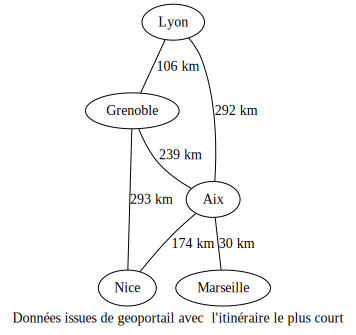
\includegraphics{reseau-routier-sud-est.png}

}

\caption{Réseau sud-Est}

\end{figure}

\begin{enumerate}
\def\labelenumi{\arabic{enumi}.}
\tightlist
\item
  Implémenter ce graphe sous la forme d'un dictionnaire de liste dans
  lequel chaque clé représente le nœud étudié et les sommets adjacents
  sont représentés sous la forme d'une liste de dictionnaires clé(sommet
  adjacent): valeur(distance).
\item
  Écrire la matrice d'adjacence et vérifier qu'elle est symétrique(on
  utilisera l'ordre alphabétique pour indexer les nœuds).
\item
  Proposer un algorithme qui renvoie tous les chemins possibles pour
  aller de Nice à Lyon sans jamais passer deux fois par la même ville.
  On utilisera trois paramètres d'entrée: le graphe implémenté sous la
  forme d'un dictionnaire d'adjacence comme celui de la question 2 et
  les deux villes de départ et d'arrivée.
\end{enumerate}



\end{document}
